\documentclass[11pt]{article}
\usepackage[final]{acl}
\usepackage{times}
\usepackage{latexsym}
\usepackage[T1]{fontenc}
\usepackage[utf8]{inputenc}
\usepackage{microtype}
\usepackage{graphicx}
\usepackage{booktabs}
\usepackage{amsmath}
\usepackage{xcolor}

% Values still to be filled from the author's own runs are shown in red.
\newcommand{\R}[1]{\textcolor{red}{#1}}
\newcommand{\tok}[1]{\texttt{#1}}

\title{Replicating and Extending LIME:\\Do Local Explanations Still Reveal Spurious Features?}

\author{Muhammad Hassan Shakoor Rana \\
  School of Computing, Macquarie University \\
  \texttt{muhammadhassanshakoor.rana@students.mq.edu.au}}

\begin{document}
\maketitle

\begin{abstract}
LIME \citep{ribeiro2016why} is an explanation algorithm that interprets a single prediction of a classifier by modelling its behaviour around the prediction as a sparse linear model. The paper makes two main claims: the explanations LIME provides are faithful to the model, and they help people to see when a model should not be trusted. I reproduce both on the original data using the library released by the authors, and test them on two other existing datasets (UCI Heart Disease and Adult Income) and on a constructed dataset of 2,000 real film reviews that I artificially add a meaningless token to at four controlled levels and a no-signal level. In the classifier-selection study, an LLM is used to represent the crowd workers of the paper. LIME recovers 97--100\% of the gold features of interpretable models, and the paper's 20 Newsgroups failure replicates closely: the original classifier falls from 94.7\% to 54.0\% on real-world pages. On new data, LIME exposes a model's reliance on a proxy for sex in Adult Income, and on the constructed data its weight tracks each model's measured reliance on the artefact ($r = 0.98$ and $0.94$). An LLM judge shown explanations in the format of the paper's crowd study picks the better classifier in 90\% of trials.

\end{abstract}

% =====================================================================
\section{Description of the Paper and Justification}
\label{sec:paper}

\citet{ribeiro2016why}\footnote{\url{https://arxiv.org/abs/1602.04938}} propose LIME (Local Interpretable Model-agnostic Explanations). To explain a prediction for an input $x$, LIME draws perturbed copies of $x$ (for text, by deleting random subsets of its words), queries the black-box model on each, and fits a weighted sparse linear model in which perturbations closer to $x$ count more. The $K$ largest coefficients are the explanation: for example, the six words that most pushed a document towards ``Atheism''. Because LIME only calls the model's \tok{predict\_proba}, it works with any classifier. The paper also proposes SP-LIME, a submodular procedure that picks a small set of instances whose explanations together cover the most important features, so that a person can judge a whole model from a few examples.

\paragraph{Evaluation framework.} The paper checks LIME in two phases. \emph{Simulated experiments} (\S5 of the paper) use classifiers whose true features are known. Sparse logistic regression and decision trees trained on books and DVD reviews rely on 10 features per instance at most, and LIME recovers more than 90\% of these (recall), much better than the greedy, Parzen, and random baselines. LIME successfully classifies untrustworthy predictions in simulated trust experiments with an $F_1$ score between 91.8 and 96.7\% (Table~1 of the paper). \emph{Human experiments} (\S6) use 20 Newsgroups. An RBF-kernel SVM achieves 94.0\% on the test split but only 57.3\% on a religion dataset the authors collected from the web, because it relies on e-mail header words such as \tok{Posting} and \tok{Host}; a manually cleaned version reaches 88.6\% and 69.0\%. Shown six explanations of six words each, Mechanical Turk users picked the cleaned classifier 89\% of the time with SP-LIME and 75\% with random picks (Figure~9 of the paper). In an image study, trust in a deliberately flawed husky-versus-wolf classifier fell from 10 of 27 graduate students to 3 of 27 after they saw explanations.

I test the paper's two claims: \textbf{C1}, LIME's explanations are \emph{faithful} to what the model actually uses; and \textbf{C2}, they let people \emph{detect untrustworthy models}, in particular reliance on spurious features.

\paragraph{Justification.} The paper appeared at KDD 2016, rated A* in the CORE ranking. In Google Scholar's Data Mining \& Analysis subcategory, KDD ranks second overall by h5-index (124) and first among conferences, behind only the journal \emph{IEEE Transactions on Knowledge and Data Engineering}. The paper has 40,713 citations on Google Scholar (accessed 4 November 2026), and its library has about 12.1k GitHub stars and 1.85k forks. The project is feasible: the code is public and pip-installable, every original text dataset is available, and the experiments run on a laptop CPU. The proposal's feasibility check ran the library successfully on Python 3.11.9.

% =====================================================================
\section{Original Datasets}
\label{sec:origdata}

\begin{table}[t]
\centering\small
\begin{tabular}{@{}lrl@{}}
\toprule
Dataset & Size & Used in paper for \\
\midrule
Books reviews & 2,000 & \S5 simulated \\
DVD reviews & 2,000 & \S5 simulated \\
20 Newsgroups (2 classes) & 1,796 & \S3, \S6 human \\
Religion web pages & 1,638 & \S6 real-world test \\
Husky/wolf images & 80 & \S6.4 (not replicated) \\
\bottomrule
\end{tabular}
\caption{Original datasets. 20 Newsgroups: 1,079 training and 717 test posts. Religion: 819 pages per class after the authors' balancing.}
\label{tab:origdata}
\end{table}

\begin{figure}[t]
\centering\scriptsize
\fbox{\parbox{0.95\columnwidth}{\ttfamily
\textbf{\rmfamily 20 Newsgroups, test post 55 (atheism)}\\
From: livesey@\ldots{} (Jon Livesey)\\
Subject: Re: A Little Too Satanic\\
Organization: sgi\\
Lines: 56\\
Distribution: world\\
NNTP-Posting-Host: solntze.wpd.sgi.com\\[2pt]
In article <\ldots>, mangoe@\ldots{} writes:\\
|> Jon Livesey writes:\\
|> |> What I said was that people took time to *copy* \ldots\\[4pt]
\textbf{\rmfamily Books review, processed (word:count, label)}\\
holes:1 must:1 top\_secret:1 he:1 center:1 other\_civilans:1 the\_pacific:1 the\_navy:1 a\_lot:1 \ldots{} \textless num\textgreater\_feet:2 \ldots{} \#label\#:positive\\[4pt]
\textbf{\rmfamily Religion dataset (rendered web page)}\\
The AHA Foundation \textbullet{} Home \textbullet{} About Us \textbullet{} Issues \ldots
}}
\caption{Format of the original text datasets (e-mail addresses masked here). Books and DVD reviews are distributed as bags of unigrams and bigrams with counts; the paper keeps only unigrams.}
\label{fig:origsnippets}
\end{figure}

Table~\ref{tab:origdata} lists the datasets. The \textbf{books and DVD} reviews come from the multi-domain sentiment corpus of \citet{blitzer2007biographies}\footnote{\url{https://www.cs.jhu.edu/~mdredze/datasets/sentiment/}}: Amazon reviews, 1,000 positive and 1,000 negative per domain. They are distributed pre-tokenised as \tok{word:count} pairs (Figure~\ref{fig:origsnippets}). Following the authors' loader, I keep unigrams, repeat each word by its count, shuffle with seed 1 and split 80/20 (1,600/400). \textbf{20 Newsgroups} \citep{lang1995newsweeder}\footnote{\url{https://scikit-learn.org/stable/datasets/real_world.html\#newsgroups-dataset}} is restricted to \tok{alt.atheism} versus \tok{soc.religion.christian}. Each post is raw e-mail text whose header block (\tok{From}, \tok{Organization}, \tok{NNTP-Posting-Host}) correlates with the label without being about religion. The \textbf{religion dataset}\footnote{\url{https://github.com/marcotcr/lime-experiments}} contains DMOZ web pages rendered to text with \tok{w3m}: 819 atheism and 1,000 Christianity pages, balanced to 819 each. It provides a test set from a different source, so header shortcuts cannot help.

% =====================================================================
\section{Replication of the Original Work}
\label{sec:replication}

\subsection{Environment and approach}
I used the authors' packaged library, \tok{lime} 0.2.0.1 (repository commit \tok{fd7eb2e}), with scikit-learn 1.9.0 and NumPy 2.4.6 on Python 3.11.9, in a virtual environment on macOS; the repository's Dockerfile and \tok{requirements.txt} pin Python and these library versions. \texttt{git status} on the clone confirms that the library source was not modified. The paper's own experiment code, in the same repository as the religion dataset (footnote~4), is frozen in Python 2 with scikit-learn 0.18 and \tok{numpy} 1.14, which no longer install on current systems, and it hard-codes a local data path. Instead of running it, I ported its logic to Python 3. This covered the classifiers, the gold-feature definitions, the greedy explainer and the data loading, and the scripts note each point where they follow the original. Two environment problems arose. macOS Python could not verify TLS certificates when downloading datasets, which I fixed by passing the \tok{certifi} bundle to every download. Running scripts from inside the cloned repository made Python import its newer source tree instead of the installed release, and that tree needs the extra dependency \tok{pyDOE2}; installing the release from PyPI and running from outside the clone avoids this. No change to LIME itself was needed. All code is in the project repository.\footnote{\url{https://github.com/Hassan-Shakoor/lime-reproducibility}}

The project uses several techniques from the unit. Scripts download every dataset from the Internet and cache it, so results can be reproduced. Data analysis and generation are scripted end to end, with fixed seeds. A virtual environment and a Docker image capture the software environment, git and GitHub hold the code and data, and the report is written in \LaTeX.

\subsection{Faithfulness (C1): recall of gold features}

\begin{table}[t]
\centering\small
\setlength{\tabcolsep}{4pt}
\begin{tabular}{@{}llrrr@{}}
\toprule
Data & Model & Random & Greedy & LIME \\
\midrule
Books & sparse LR & 20.3 (17.4) & 78.0 (64.3) & 100.0 (92.1) \\
      & tree      & 20.0 (20.6) & 55.6 (37.0) & 98.5 (97.0) \\
DVDs  & sparse LR & 20.2 (19.2) & 74.0 (63.4) & 100.0 (90.2) \\
      & tree      & 18.4 (17.4) & 59.3 (47.6) & 97.4 (97.8) \\
\bottomrule
\end{tabular}
\caption{Recall (\%) of gold features with $K=10$, averaged over the 350--372 test reviews per setting that have gold features: replicated value, with the paper's value (Figures~6--7) in brackets. Parzen is omitted because the library does not implement it.}
\label{tab:recall}
\end{table}

Again as in \S5.2 of the paper, there are two interpretable classifiers. The first one is logistic regression with L1 regularisation, where the regularisation coefficient $C$ is reduced from 0.1 by 0.01 until it ensures that no training review has more than 10 words used with a non-zero weight. The second is a decision tree. The gold features for a test review are the words that do not have weights of zero in the LR (non-zero weight words) or the words that are tested on the decision path of the tree (words on decision path). Each explainer contributes $K = 10$ words, and recall is the share of gold words recovered. LIME uses K-Lasso feature selection, as in the paper, with 5,000 perturbation samples rather than the paper's 15,000, to fit a laptop budget.

Table~\ref{tab:recall} shows that the claim replicates. LIME recovers 97.4--100\% of gold features, matching or exceeding the paper's values to within 0.4 points. The ordering LIME $>$ greedy $>$ random holds in all four settings, random stays near 20\% as in the paper, and greedy again falls well behind LIME on decision trees. Greedy achieves a higher score than in the paper on all four settings (10.6--18.6 points higher) and LIME is higher on sparse LR (100\% vs.\ 92.1\% and 90.2\%). The classifier, not the explainer, is the most likely culprit for sparse LR. With current scikit-learn, the first $C$ satisfying the 10-feature cap is 0.03, yielding very sparse models: 7 (books) and 11 (DVD) non-zero words in total, with test accuracy 67\% and 65\%. Thus each review has on average only 2.3 gold words and 3.0 gold words, which is an easier target than the models in the paper probably saw. On decision tree models (whose gold sets average 1.4--1.5 words), LIME and random closely follow the paper. The higher greedy scores there suggest that my unpruned trees (depth 61) differ from the paper's. Other differences include fewer perturbation samples (5,000 instead of 15,000) and the library's default kernel width rather than a cross-validated one. I did not test their effect separately, but LIME's recall is not lower than the paper's despite them.

\subsection{Detecting untrustworthy models (C2): 20 Newsgroups}

\begin{table}[t]
\centering\small
\begin{tabular}{@{}lrrrr@{}}
\toprule
& \multicolumn{2}{c}{20NG test} & \multicolumn{2}{c}{Religion} \\
\cmidrule(lr){2-3}\cmidrule(lr){4-5}
Classifier & ours & paper & ours & paper \\
\midrule
Original SVM & 94.7 & 94.0 & 54.0 & 57.3 \\
Cleaned SVM  & 80.3 & 88.6 & 57.7 & 69.0 \\
Naive Bayes (original) & 95.4 & -- & 56.2 & -- \\
\bottomrule
\end{tabular}
\caption{Accuracy (\%) on the 20 Newsgroups test split and on the religion dataset. ``Cleaned'' removes headers, footers and quotes, an automatic stand-in for the paper's manual feature removal.}
\label{tab:religion}
\end{table}

As in the paper, I used an RBF kernel SVM classifier with TF-IDF features, and tuned the $C$ and $\gamma$ parameters with 3-fold cross-validation. The cleaned classifier in the paper was produced manually by removing words that do not generalise. The reproducible version of mine was done by stripping every post's header, signature and quoted lines with the \tok{remove} option of scikit-learn. Table~\ref{tab:religion} compares the two. The central result replicates closely. The original SVM ($C = 100$, $\gamma = 0.1$) scores 94.7\% on the 20NG test split, against the paper's 94.0\%, but only 54.0\% on the religion pages, against 57.3\%. That 40.7-point collapse is close to the paper's 36.7, and the Naive Bayes classifier from the feasibility check behaves the same way. Cleaning moves in the paper's direction but by less: religion accuracy rises 3.7 points rather than 11.7, while 20NG accuracy falls 14.4 points rather than 5.4. Removing entire header, signature and quote blocks removes topical content as well as the artefacts (replies in quotes often contain the argument). The paper’s manual cleaning removed only selected words. The cleaned classifier is therefore better in the real world, as in the paper, but by a smaller margin.

I then ran LIME with $K = 6$ as in \S6.2 on both classifiers on 100 random test posts (96 for the cleaned one, as four posts are empty after removing headers). The following statistics are for the original classifier: 14.3\% of all explanation words are only in the header block of the post, and in 41\% of posts at least one of the six explanation words comes only from the header. By construction, this figure is 0\% for the cleaned classifier, as there is no header in its input. A worked example shows the effect. In the proposal's feasibility run on test post~83, a Naive Bayes classifier predicted ``atheism'' with probability 0.576, and LIME's three strongest words were \tok{Host} ($-0.158$), \tok{Posting} ($-0.150$) and \tok{NNTP} ($-0.090$). All three are header words, and the negative weights mean each pushed the prediction away from ``christian''. The prediction is barely confident, and the explanation shows it rests on the message's routing metadata rather than on its content. This is exactly the failure LIME is meant to reveal.

\paragraph{Where LIME works and where it does not.} The clearest success is test post 193, whose body is empty. The original classifier still predicts ``atheism'' with probability 0.98, and LIME attributes it to \tok{Host} (+0.23), \tok{Posting} (+0.22) and \tok{Nntp} (+0.18): the decision is visibly made by routing metadata. On post 79 the original classifier is correct because of \tok{uk}, \tok{Posting}, \tok{Host} and \tok{Nntp}, while the cleaned one is correct on content words such as \tok{religion}. Both are right, but only LIME shows that one of them is right for the wrong reason, which accuracy alone cannot reveal. Post 85 shows that the leakage is not limited to headers. The original classifier's top words are \tok{wwc}, \tok{saturn} and \tok{healta}, fragments of an e-mail address in the attribution line of a quoted reply (``In article \ldots{} writes:''). LIME's limits show on post 156, an atheist's post quoting Genesis. Both classifiers predict ``christian'' on \tok{God} and \tok{earth}, words a user would find reasonable, yet the prediction is wrong. LIME is faithful to the model rather than to the truth, so a plausible explanation does not certify a correct prediction.

\paragraph{Not replicated.} The Mechanical Turk studies (\S6.2--6.3) would need paid crowd workers and ethics approval; \S\ref{sec:llmjudge} substitutes an LLM judge for \S6.2. The husky/wolf study (\S6.4) depends on 80 hand-picked images and a trained network that were not released, and it involved human subjects. The simulated trust experiments (\S5.3--5.4) reuse the same books/DVD models as \S5.2 and add no new data source, so I prioritised the real-world shift test above.

% =====================================================================
\section{Construction of New Data}
\label{sec:newdata}

Following the proposal, I applied LIME to two new existing datasets and built one new dataset. The proposal listed five candidates. Three were dropped: Credit Card Fraud and Jigsaw Toxic Comments need a Kaggle account and licence acceptance that a marker could not reproduce automatically, and IMDB is a large download whose sentiment task overlaps with the constructed data.

\paragraph{Heart Disease (Cleveland).} This UCI dataset \citep{detrano1989international}\footnote{\url{https://archive.ics.uci.edu/dataset/45/heart+disease}} has 303 patients and 13 clinical attributes, distributed as comma-separated values with \tok{?} for missing entries (Figure~\ref{fig:newsnippets}). Six values were missing (4 in \tok{ca}, 2 in \tok{thal}) and were median-imputed. The 0--4 severity target was binarised to absent (164) versus present (139). Seven attributes are categorical codes (\tok{sex}, chest-pain type \tok{cp}, \tok{fbs}, \tok{restecg}, \tok{exang}, \tok{slope}, \tok{thal}) and were declared as such to LIME, so that explanations read ``\tok{cp=4}'' rather than as a threshold on a code number.

\paragraph{Adult Income.} The UCI Adult census extract \citep{kohavi1996scaling}\footnote{\url{https://archive.ics.uci.edu/dataset/2/adult}} predicts whether income exceeds \$50K. After merging the train and test files and dropping rows with missing values, 45,222 people remain (24.8\% positive). I dropped \tok{fnlwgt}, a census sampling weight rather than a property of the person, and integer-coded and declared the eight categorical attributes. The dataset contains the sensitive attributes \tok{sex} and \tok{race}, plus \tok{relationship}, which encodes sex through ``Husband''/``Wife''. It therefore tests C2 in a fairness setting: does LIME show when a model leans on protected attributes?

\paragraph{Constructed dataset: real reviews with a controlled artefact.} The update presentation used 300 templated sentences; following its feedback, the final dataset uses real text. The base corpus is the polarity dataset v2.0 of \citet{pang2004sentimental}\footnote{\url{https://www.cs.cornell.edu/people/pabo/movie-review-data/}}: 2,000 IMDb film reviews, 1,000 positive and 1,000 negative, labelled from the reviewers' star ratings and averaging about 700 words. Into these I inject a spurious feature whose presence and strength are known exactly, which the paper's 20 Newsgroups headers do not allow. For each of five seeds, a stratified 80/20 split is made and the meaningless token \tok{zzqref} is attached as a final line, somewhat like a forum signature, to a selected portion of the reviews in train and test. There are five conditions (Table~\ref{tab:conditions}). In the four \emph{negative} conditions, the token is only added to negative reviews, to 100\%, 75\%, 50\% or 25\% of them. So whenever the token appears the review is negative, but it appears in fewer and fewer of the negative reviews. In the \emph{control} it appears in half of all reviews independent of label, so it carries no signal. This gives $5\times5 = 25$ dataset versions. A manifest of 50,000 rows records every review's split and injection status, and the seed-0 versions are stored in full in the repository, with a datasheet in the style of \citet{gebru2021datasheets}.

\begin{table}[t]
\centering\small
\begin{tabular}{@{}lrrr@{}}
\toprule
Condition & neg.\ & pos.\ & P(neg $\mid$ token) \\
\midrule
neg100 & 100\% & 0\% & 1.0 \\
neg75 & 75\% & 0\% & 1.0 \\
neg50 & 50\% & 0\% & 1.0 \\
neg25 & 25\% & 0\% & 1.0 \\
control & 50\% & 50\% & 0.5 \\
\bottomrule
\end{tabular}
\caption{Injection conditions: share of negative and positive reviews carrying the token, applied identically to train and test splits.}
\label{tab:conditions}
\end{table}

\begin{figure}[t]
\centering\scriptsize
\fbox{\parbox{0.95\columnwidth}{\ttfamily\raggedright
\textbf{\rmfamily Heart Disease (one row, target last)}\\
63.0,1.0,1.0,145.0,233.0,1.0,2.0,\allowbreak 150.0,0.0,2.3,3.0,0.0,6.0,0\\[4pt]
\textbf{\rmfamily Adult Income (one row)}\\
39, State-gov, 77516, Bachelors, 13, Never-married, Adm-clerical, Not-in-family, White, Male, 2174, 0, 40, United-States, {<=}50K\\[4pt]
\textbf{\rmfamily Constructed review, neg100 (end of text)}\\
\ldots{} whatever . . . skip it ! where's joblo coming from ?\\
a nightmare of elm street 3 ( 7/10 ) - blair witch 2 ( 7/10 ) - \ldots{} - stir of echoes ( 8/10 )\\
zzqref
}}
\caption{Snippets of the new data. The constructed review (\tok{cv000\_29416}, negative) already ends with the reviewer's signature line of ratings, a natural artefact of the kind the injected token imitates.}
\label{fig:newsnippets}
\end{figure}

\paragraph{Annotation and data quality.} No new human labels were needed: the sentiment labels are the original corpus's rating-derived labels, and the injection adds a token without altering any review text, so the labels remain valid by construction. The constructed data thus matches the original reviews in quality and exceeds them in one respect: the ground truth about the spurious feature is known, rather than inferred as it is with the 20 Newsgroups headers.

% =====================================================================
\section{Results on New Data}
\label{sec:results}

\subsection{Heart Disease and Adult Income}

Both datasets use a random forest, with five stratified 80/20 splits (seeds 0--4). For every explained test instance (all 61 test patients for Heart Disease; 200 people for Adult), I record which features fall in LIME's top five. Two checks follow. \emph{Aggregate faithfulness}: does the frequency with which features appear in local explanations agree with the forest's global permutation importance (Spearman $\rho$)? \emph{Stability}: for 20 instances, LIME is rerun with five different sampling seeds on the same model; I report the mean pairwise Jaccard overlap of the top-five sets and how often each rerun's top feature agrees with the first run's (measured on the seed-0 split).

\begin{figure*}[t]
\centering
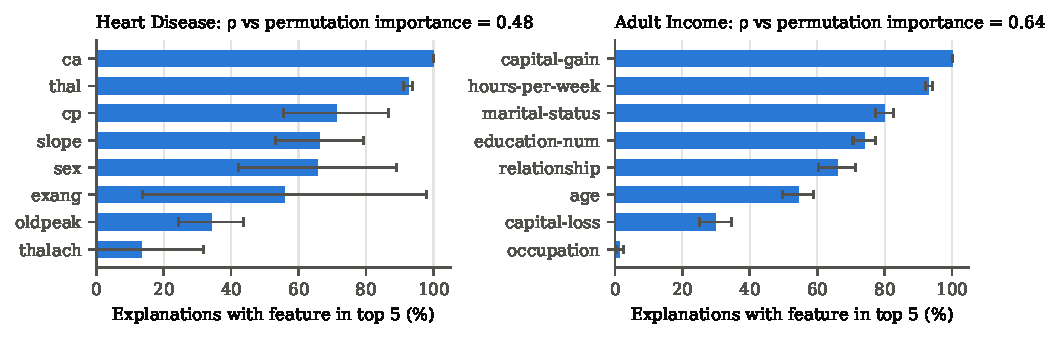
\includegraphics[width=0.9\textwidth]{figures/tabular.pdf}
\caption{How often the eight most frequent features appear in LIME's top five, averaged over five splits (error bars: sd). Titles give the Spearman correlation with permutation importance.}
\label{fig:tabular}
\end{figure*}

\paragraph{Heart Disease.} The forest reaches $85.2 \pm 2.7\%$ accuracy (range 82.0--90.2\%). The single split shown in the project update (91.8\%, a different random split) lies above this range, which illustrates why the final evaluation uses five. LIME's explanations are dominated by established clinical markers: the number of vessels coloured by fluoroscopy (\tok{ca}, in 100\% of top-five lists), the thallium stress test (\tok{thal}, 92.5\%) and chest-pain type (\tok{cp}, 71.1\%). Age and cholesterol almost never appear (0\% and 0.3\%). Agreement with permutation importance is positive on average ($\rho = 0.48$) but varies widely across splits, from $-0.19$ to $0.84$. With only 61 test patients, permutation importance is itself noisy, and correlated features trade places between models: \tok{exang} appears in $56 \pm 42\%$ of lists depending on the split. Repeated LIME runs on the same patient overlap well (Jaccard 0.84) but name a different top feature one time in four (top-1 agreement 0.75), so a single explanation of a single patient should not be over-read.

\paragraph{Adult Income.} The forest reaches $84.7 \pm 0.1\%$. Explanations agree well with permutation importance ($\rho = 0.64 \pm 0.06$) and are very stable (Jaccard 0.92, top-1 agreement 1.00). The most frequent features are \tok{capital-gain} (100\%), \tok{hours-per-week} (93.1\%) and \tok{marital-status} (79.9\%). The fairness finding is subtler than expected. The protected attributes themselves rarely appear: \tok{sex} in 1.1\% of explanations and \tok{race} in none. But \tok{relationship}, whose ``Husband'' and ``Wife'' values encode sex, appears in 65.9\%; in the example explanations, \tok{relationship=Husband} pushes predictions towards $>$\$50K. LIME thus exposes reliance on an attribute that partly encodes sex, which an audit checking only the \tok{sex} column would miss; this supports C2 in a setting the paper did not test. The attribute is confounded with marriage, and \tok{marital-status} (79.9\%) carries similar information, so LIME shows \emph{where} to look rather than proving discrimination. A model without \tok{sex}, \tok{race} and \tok{relationship} loses only about 0.25 points ($84.4 \pm 0.2\%$), though it can still use \tok{marital-status}.

\subsection{Constructed dataset}

\begin{figure*}[t]
\centering
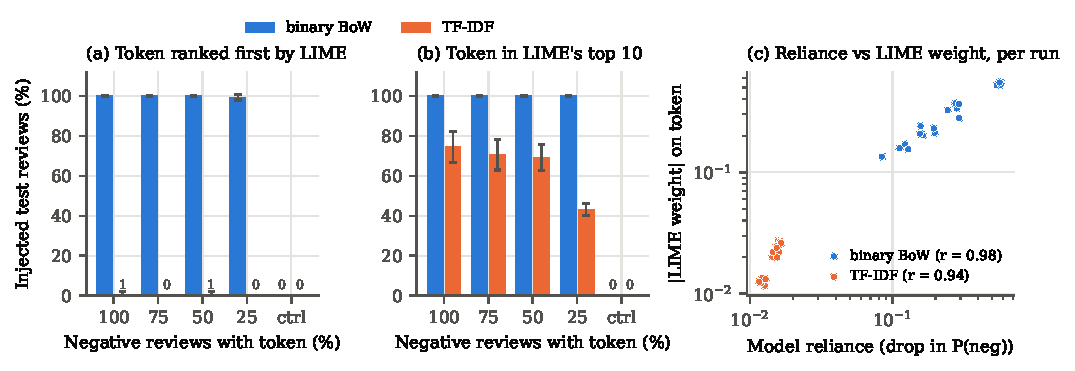
\includegraphics[width=\textwidth]{figures/constructed.pdf}
\caption{Constructed dataset, binary bag-of-words versus TF-IDF models. (a, b) Share of injected test reviews in which LIME ranks the token first or in its top ten (mean $\pm$ sd over 5 seeds). (c) Each non-control run: the model's measured reliance on the token against LIME's mean weight for it (log scales).}
\label{fig:constructed}
\end{figure*}

% Numbers from results/constructed_binary.json and results/constructed_tfidf.json
% (5 seeds per condition; mean, with sd in Figure 3).
\begin{table}[t]
\centering\small
\setlength{\tabcolsep}{3.5pt}
\begin{tabular}{@{}llrrrrr@{}}
\toprule
& & \multicolumn{2}{c}{Accuracy (\%)} & Reliance & \multicolumn{2}{c}{LIME (\%)} \\
\cmidrule(lr){3-4}\cmidrule(lr){6-7}
Model & Cond. & token & clean & $\Delta$P & top-1 & top-10 \\
\midrule
Binary & neg100 & 99.6 & 67.2 & .568 & 100 & 100 \\
       & neg75  & 92.6 & 82.6 & .278 & 100 & 100 \\
       & neg50  & 89.9 & 86.2 & .174 & 100 & 100 \\
       & neg25  & 87.9 & 86.5 & .107 & 99.3 & 100 \\
       & control& 86.4 & 86.4 & .003 & 0 & 0 \\
\midrule
TF-IDF & neg100 & 84.5 & 82.5 & .016 & 0.7 & 74.7 \\
       & neg75  & 83.9 & 82.5 & .016 & 0 & 70.7 \\
       & neg50  & 83.5 & 82.6 & .015 & 0.7 & 69.3 \\
       & neg25  & 83.2 & 82.8 & .012 & 0 & 43.3 \\
       & control& 82.8 & 82.8 & .001 & 0 & 0 \\
\bottomrule
\end{tabular}
\caption{Constructed dataset, mean of 5 seeds. Accuracy on the test split as built (``token'') and with the token removed (``clean''). $\Delta$P: mean drop in P(negative) when the token is deleted from an injected review. LIME: share of 30 injected test reviews per seed in which the token is ranked first or in the top ten.}
\label{tab:constructed}
\end{table}

Each of the 50 runs (2 models $\times$ 5 conditions $\times$ 5 seeds) trains a logistic regression, and LIME ($K = 10$, 2,000 samples) then explains 30 injected test reviews. I used two feature representations to obtain models that rely on the artefact to very different degrees. In \emph{binary} bag-of-words the token counts as much as any other word. In \emph{TF-IDF}, length normalisation dilutes one token among about 700. Because the models are linear, their true reliance is measurable: the drop in P(negative) when the token is deleted ($\Delta$P).

Table~\ref{tab:constructed} and Figure~\ref{fig:constructed} give the results. \textbf{The binary model reproduces the paper's 20 Newsgroups failure in a controlled form.} When every negative review carries the token, the model scores 99.6\% with it but 67.2\% once it is removed, the same kind of collapse as the original SVM's drop from the 20NG test split to the religion pages. LIME ranks the token \emph{first} in 100\% of these reviews, and still in 99.3\% when only a quarter of negative reviews carry it. In the control, where the token predicts nothing, LIME never lists it. \textbf{The TF-IDF model shows the converse.} The token is that model's largest or near-largest coefficient (largest at neg100 and neg75, third at neg25), yet deleting it changes a prediction by only 0.016, and accuracy with and without it differs by at most 2 points. LIME again reflects this: it almost never ranks the token first, but lists it in the top ten 69--75\% of the time, falling to 43\% at the weakest condition. Across the 20 non-control runs per model, LIME's weight on the token tracks the measured reliance (Pearson $r = 0.98$ binary, $0.94$ TF-IDF; Figure~\ref{fig:constructed}c). For TF-IDF the reliance spans only 0.012--0.016, so that correlation mainly separates the weakest condition from the rest (within neg100--neg50, $r = 0.64$).

These results support both claims on new data. LIME is faithful (C1): its weight follows how much each model actually uses the artefact, not how strongly the artefact correlates with the label in the data, since the label correlation is identical for the two models. It also supports detecting untrustworthy models (C2): whenever the model relies heavily on the artefact (binary neg100, losing 32 accuracy points without it), LIME ranks the artefact first. LIME tracks reliance rather than the accuracy cost, so it also ranks the token first at binary neg25, where removing it costs only 1.4 points; judging whether a flagged feature matters still needs a held-out check. The evaluation goes beyond the replication in one respect. The paper could only \emph{show} that header words appear in explanations; here the size of the spurious effect is known, so LIME's sensitivity can be measured as a function of it.


\subsection{LLM-as-judge}
\label{sec:llmjudge}

For the subjective trust judgements I replace the paper's own experiment (\S6.2) with an LLM judge, as proposed by \citet{zheng2023judging}; this is justified because trust judgements are subjective, while the answer to the recall experiment is computable. In 40 trials, the judge, \tok{gpt-5-mini}, sees information in the same format as the paper’s crowd workers: six documents, each with the predictions of both classifiers and their six strongest words marked as “supports” or “opposes”. The judge is asked which classifier will be more accurate on web pages about religion. The six documents are chosen either by SP-LIME or at random, from a pool of 50 explained test posts; in every trial, the two classifiers are randomly called A and B. The right answer is the cleaned classifier, and on the religion data my replication also finds it the more accurate (Table~\ref{tab:religion}).

\begin{table}[t]
\centering\small
\begin{tabular}{@{}lrrr@{}}
\toprule
Pick method & LLM judge & 95\% CI & Humans \\
\midrule
Random (RP)     & 95.0 (19/20) & 76.4--99.1 & 75 \\
Submodular (SP) & 85.0 (17/20) & 64.0--94.8 & 89 \\
All trials      & 90.0 (36/40) & 76.9--96.0 & -- \\
\bottomrule
\end{tabular}
\caption{Share of trials (\%) in which the judge chose the cleaned classifier, with Wilson 95\% intervals, against the paper's Mechanical Turk users (Figure~9 of \citealp{ribeiro2016why}).}
\label{tab:judge}
\end{table}

The judge selected the cleaned classifier in 36 of 40 trials (90\% compared to the 50\% expected by chance; 2-sided binomial test, $p < 10^{-6}$; random choice $p < 10^{-4}$, SP $p = 0.003$), as shown in Table~\ref{tab:judge}. Whether the cleaned classifier is labelled A or B, the judge is right in 18 of 20 trials. To test directly for position bias, I repeated all 40 trials, but with A and B labels reversed. The judge was right in 35 of 40 trials (87.5\%), gave the same answer in both orders in 33 (82.5\%), and was correct in both orders in 32. The outcome is therefore not due to an artefact of label position. This is in line with C2 with a non-human reader: the judge selected the classifier with better generalisation from 6 explanations of 6 words, despite the cleaned classifier being less accurate on the held out 20NG split (80.3\% versus 94.7\%) and only slightly better on the religion pages (57.7\% vs 54.0\%). The stated reasons are consistent with the explanation in the paper of why the original classifier fails. A typical rationale reads: ``Classifier A relies more on topical religious words (Christ, sin, God, believe, coming) while B leans on forum/metadata cues (Nntp, Host, Posting, user names, uk) that won't generalize to web pages.'' One result is different from the paper. It helped humans (89\% vs 75\%) but not the judge (85\% vs 95\% for random picks): submodular pick. The condition overlaps considerably with 20 trials each, and the difference is not significant (Fisher's exact test, $p = .60$) and thus these results point to no detectable difference rather than a reversal. SP may assist in locating a few documents that together cover the important features, thus saving time in reading. That is no problem for a model that reads all words.

The evaluation differs from the replicated study in five ways: one LLM instead of 100 crowd workers, so the variability of human judgement is absent; automatic rather than manual cleaning, which leaves a smaller real-world gap between the classifiers; pools of 50 drawn from the 96 posts explained for both classifiers, rather than the full test set; the judge sees a 200-character extract of each document's header-free body, so header words appear only in the explanations, rather than the full post; and the model accepts only its default sampling temperature (it rejected temperature 0), so a rerun may differ slightly. The prompt also asks for the verdict before the reasoning; \citet{zheng2023judging} instead propose chain-of-thought judging, in which the model reasons before giving its verdict, so the stated rationales may justify the verdict rather than produce it. Finally, the judge was not validated against human labels on the same prompts (for example with Cohen's $\kappa$); that check is the natural next step before an LLM judge replaces people. All 40 prompts and replies are saved in the repository, so the scoring can be reproduced exactly.

% =====================================================================
\section{Ethical Considerations}
\label{sec:ethics}

\paragraph{In the original paper.} The \S6 studies involved human participants: 27 graduate students and Mechanical Turk workers. The paper does not report ethics approval, consent procedures or worker pay. Pay matters because earnings from crowd-work are often below minimum wage. A study of 2,676 Mechanical Turk workers found a median of about \$2 per hour, with only 4\% earning more than the US federal minimum of \$7.25 \citep{hara2018data}. These studies need to be ethically reviewed, and require informed consent and fair payment as outlined by the Australian Code for the Responsible Conduct of Research \citep{nhmrc2018code} and the National Statement \citep{nhmrc2023national}. The husky/wolf study was also deliberately deceptive: subjects were not told the classifier was built to fail. Deception can be justified in a debriefed, low-risk study, but the National Statement requires it to be explicitly approved and justified. The paper does model good practice in open science: it released its code, the religion dataset it collected and a usable library, which is what made this replication possible.

\paragraph{In this project.} The \textbf{Heart Disease} data are real patient records. They were de-identified and released for research decades ago, but they remain health information, and the original patients could not have consented to every future use. A publication should use them only for methodological purposes, cite their provenance, and make no clinical claims: an 85\% accurate forest evaluated on 61 test patients says nothing about safe diagnosis. Sex is among the model's most frequent features (65.6\% of explanations), which may reflect real clinical risk but would need scrutiny before any use. The \textbf{Adult} data contain sex and race. My results show that explanations can surface a model's reliance on such attributes, and on proxies such as \tok{relationship}, which is useful for auditing. The 20 Newsgroups posts are public but contain real names and e-mail addresses, so Figure~\ref{fig:origsnippets} masks addresses. Explanations can also be gamed: \citet{slack2020fooling} build classifiers that behave unfairly yet produce innocent-looking LIME explanations. A clean explanation should therefore never be presented as proof of fairness (``fairwashing''). The \textbf{constructed} data add only a meaningless token to publicly released reviews, so the main obligations are honest documentation and attribution, which the datasheet covers. More broadly, the instability measured in \S\ref{sec:results} means a single explanation can mislead; responsible use reports variation across seeds rather than one convenient run. All code, generated data, seeds and results, including the failed or weaker results, are public in the project repository, in line with the Code's principles of honesty, rigour and transparency. Generative AI assisted with code and drafting; all reported numbers were verified against the scripts' output files, including an independent review pass, and I read the cited works.

% =====================================================================
\section{Conclusions and Reflections}
\label{sec:conclusion}

Replication was mostly successful. After porting the authors' Python 2 experiment code, the released library ran unmodified on current software. The faithfulness result (C1) was replicated, with LIME achieving a recall of 97--100\%, matching or exceeding that of the paper. The motivating failure of the paper was closely replicated: an SVM that is 94.7\% accurate on 20 Newsgroups drops to 54.0\% on real-world pages, and LIME's explanations show why. Automatic cleaning helped less than the paper's manual cleaning, and the crowdsourced and image studies could not be repeated without paid participants or unreleased materials.

The claims generalise to new data, with two caveats. On Adult Income, LIME uncovered a model's use of a sex proxy. Furthermore, in the controlled experiment its weight on the injected token correlated with the model’s measured reliance ($r = 0.98$ for the binary model and $0.94$ for TF-IDF, across injection strengths): LIME gave the token a high weight when the model relied on it heavily, and a low weight when the model barely used it. The caveats are that small datasets make individual explanations unstable (Heart Disease top-1 agreement 0.75), and that a faithful explanation can still look plausible for a wrong prediction. Finally, an LLM judge identified the better classifier from explanations in 90\% of trials, comparable to the paper's crowd workers (95\% versus their 75\% with random picks, 85\% versus 89\% with SP), though unlike them it did not benefit from submodular pick.

\paragraph{Reflections.} The templated reviews of the project update made the artefact look more powerful than it is in real text. On real 700-word reviews, a TF-IDF model barely uses a perfectly predictive footer token, and LIME correctly reported weak influence. The \emph{model's} reliance, not the data's correlation, is what an explanation can be expected to reveal, and designing the experiment around measured reliance rather than injection rate was the most important change. Computer science is not immune to the replication problems documented in other empirical fields \citep{cockburn2020threats}; that a 2016 result could be re-run at all is owed to the released code and data. Second, porting the authors' frozen code was faster and more informative than reviving its 2016 environment, but it means small numerical differences are unavoidable. Finally, an LLM judge is cheap and repeatable, but it is a model judging a model. Its agreement with the paper's humans is evidence about the judge as much as about LIME.

\bibliography{custom}

\end{document}
